\chapter{Introduction}
Massive U(1) vector bosons, also known as heavy photons, are a natural consequence of many theories of physics beyond the Standard Model, and a basic component of many hidden sector models of dark matter.
Such a particle would kinetically mix with the photon, giving it an effective coupling to electric charge much smaller than the photon's direct coupling $\alpha$.
The existence of such a heavy photon is a possible explanation for cosmic ray anomalies and the muon $g-2$ anomaly, both of which are discussed in Section \ref{sec:motivating_observations}.
Multiple current and proposed experiments are dedicated to the search for a heavy photon, and are summarized in Section \ref{sec:searches_overview}.
%The theoretical background, physics motivation, and 

The Heavy Photon Search experiment (HPS) is designed to produce heavy photons by sending the electron beam of Jefferson Lab's CEBAF accelerator through a fixed target.
The detector is a compact, large-acceptance forward spectrometer comprising a silicon microstrip tracker (silicon vertex tracker, or SVT) for momentum measurement and vertexing and an electromagnetic calorimeter (ECal) for triggering.
The experiment has recorded physics data in 2015 and 2016, with future running scheduled.

The properties of a heavy photon are described by the heavy photon mass $m_{A'}$ and the dimensionless kinetic mixing strength $\epsilon$; the coupling to electric charge scales with $\epsilon^2$ and therefore it is common to quote results in terms of $\epsilon^2$.
$\epsilon^2$ also equals $\alpha'/\alpha$, the ratio between the heavy photon coupling to charge and the photon coupling to charge.
Figure \ref{fig:reach} shows current constraints in this parameter space from other experiments, and the projected HPS reach as presented in the 2014 HPS proposal \cite{collaboration_heavy_2013}.

\begin{figure}[ht]
    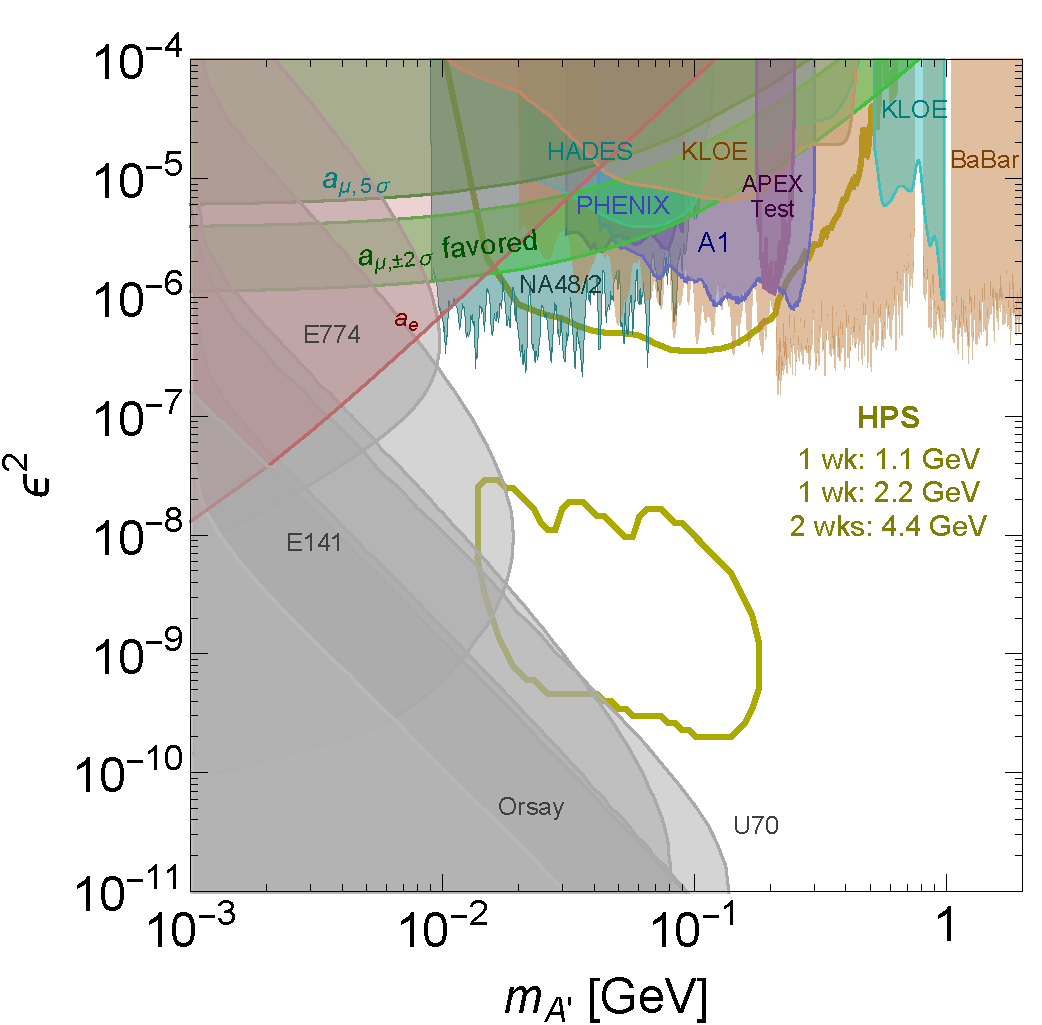
\includegraphics[width=\textwidth]{intro/figs/A-visible-HPS-official-6-2015}
    \caption{The yellow-green contours outline the expected reach (for exclusion at 90\% confidence level) for the HPS experiment with the run plan shown.
    The reach is split in two regions; the upper region corresponds to the bump-hunt and the lower region corresponds to the vertexing search.
    Existing limits from other experiments are plotted as shaded regions.
    The favored region from the muon $g-2$ anomaly is plotted as a shaded green band (upper left).}
    \label{fig:reach}
\end{figure}

If produced at HPS, heavy photons will decay to $e^+e^-$ pairs, possibly with some finite decay length; the HPS detector measures the momentum and decay vertex of the pairs.
The invariant mass and vertex of the pairs are used in two searches for heavy photons, covering different regions of the parameter space: a ``bump-hunt'' and a vertexing search.
The bump-hunt is a search for a narrow mass resonance above a smooth background, and is sensitive to heavy photons with relatively large couplings (and hence large production).
The vertexing search is a search for $e^+e^-$ pairs produced downstream of the target, and is sensitive to heavy photons with relatively small couplings (and hence long decay lengths).
This dissertation presents the vertexing search.

The 2015 HPS run was at a beam energy of 1.056 GeV, and nominal current of 50 nA.
The beam charge collected during physics data-taking is summarized in Figure \ref{fig:beamtime}.
Because detector commissioning was in progress throughout the run, the SVT was not moved to its nominal position (0.5 mm from the beam) until late in the run.
Roughly comparable amounts of data were recorded with the SVT at 1.5 mm and 0.5 mm from the beam.

This dissertation uses only the 2015 data from operation at 0.5 mm.
A total of 1166 nb$^{-1}$ of good data was recorded under these conditions, from May 13 through May 18.
This value is corrected for trigger deadtime and run quality, as described in Section \ref{sec:luminosity}; it is equivalent to 1.69 days of ideal running at the nominal beam current.
Approximately 90\% of the data was blinded so detector performance studies and analysis development could be done on the other 10\% without biasing the ultimate result.
This dissertation uses only the unblinded fraction, which is a total of 119 nb$^{-1}$ (0.172 days equivalent).

\begin{figure}[ht]
    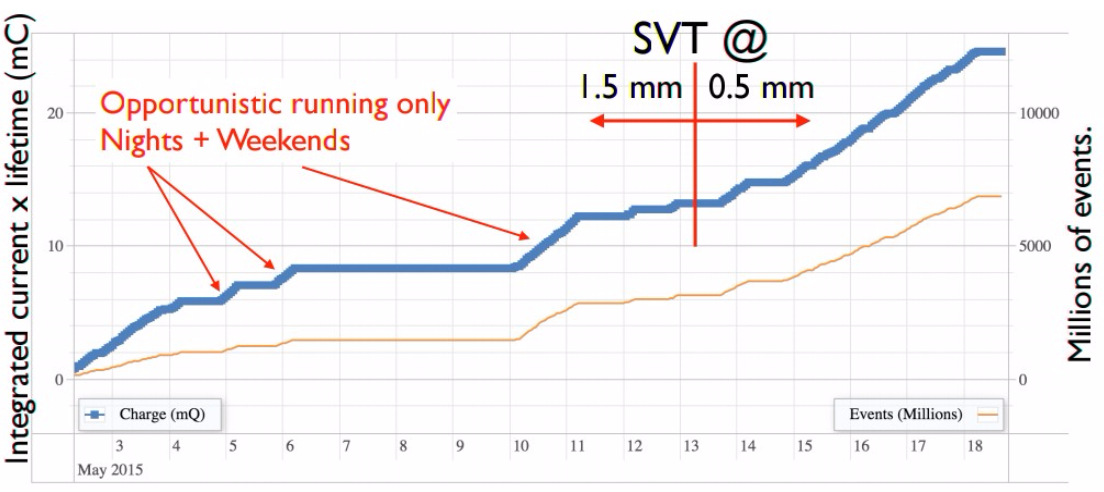
\includegraphics[width=\textwidth]{intro/figs/engrun-beamtime}
    \caption{Rough totals for integrated charge and event count during the 2015 HPS run. The numbers in this plot are not fully corrected for run and event quality.}
    \label{fig:beamtime}
\end{figure}

This dissertation presents the HPS experiment as a whole without specific reference to my personal contributions; those are summarized here.
I was responsible for the survey of the SVT, and assembled the modules and U-channels (both described in Section \ref{sec:svt_mechanical}).
I installed and documented the SVT cooling systems described in Section \ref{sec:svt_services}.
I developed the hit time reconstruction algorithm used in the SVT, described in Section \ref{sec:svt_hit_recon}.
I developed the detector readout and trigger simulations, which fully simulate the detector pileup, time evolution of pulses and readout pipelines, and trigger algorithms.
I used this trigger simulation for the performance studies and tuning of trigger parameters presented in the 2014 HPS proposal; the final trigger parameters described in Section \ref{sec:trigger_cuts} are based on that work.


Finally, I have had primary responsibility for the displaced-vertex search.
The analysis presented in Chapter \ref{sec:vertexing} was outlined in the 2014 HPS proposal \cite{collaboration_heavy_2013}, but I implemented it.
Section \ref{sec:proposal_reach} discusses differences between the proposal outline of the analysis, and what I have done.